\documentclass{standalone}

\begin{document}


\begin{frame}{The Big Data era}{Data generation in Real Time}

  \centering Big Data are the new microscopy to \quotes{measure} the society.

  \vspace{0.3cm}

  \centering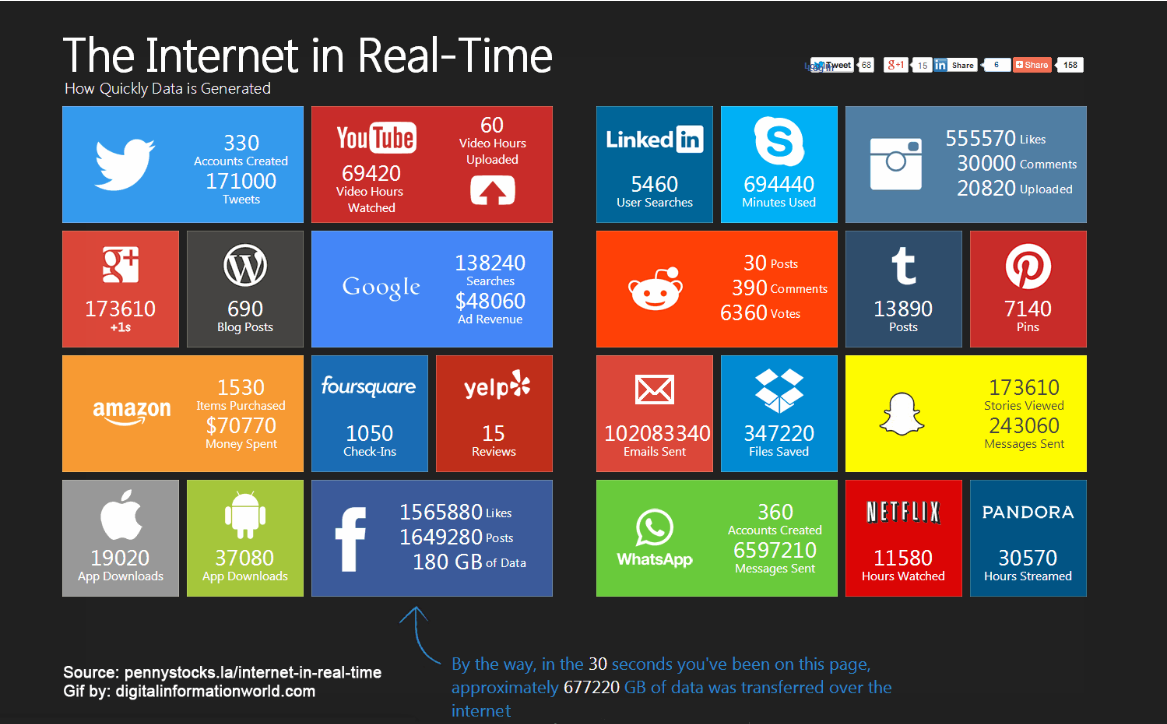
\includegraphics[width=0.9\textwidth]{./big_data_real_time.png}

\end{frame}



\begin{frame}{The 5 V's of Big Data}{Big Data characteristics}

  \setbeamertemplate{itemize items}[ball]
  \setbeamertemplate{itemize/enumerate body begin}{\scriptsize}
  \setbeamertemplate{itemize/enumerate subbody begin}{\scriptsize}

  \begin{columns}
    \begin{column}{0.5\textwidth}

      \begin{itemize}
        \setlength\itemsep{1em}

        \item \textbf{Volume}: Terabytes to exabytes of existing data to process.

        \item \textbf{Velocity}: Streaming data, requiring msec to respond.

        \item \textbf{Variety}: different types of data we can now use $\xrightarrow{}\begin{cases}Structured\ data\\Semi-Structured\ data\\Unstructured\ data
        \end{cases}$

        \item \textbf{Veracity}: Uncertainty due to data inconsistency \& incompleteness, ambiguities, latency, deception.

        \item \textbf{Value}: \textcolor{red}{It is all well and good having access to big data but unless we can turn it into value it is useless}.
      \end{itemize}
    \end{column}

    \begin{column}{0.4\textwidth}
      \centering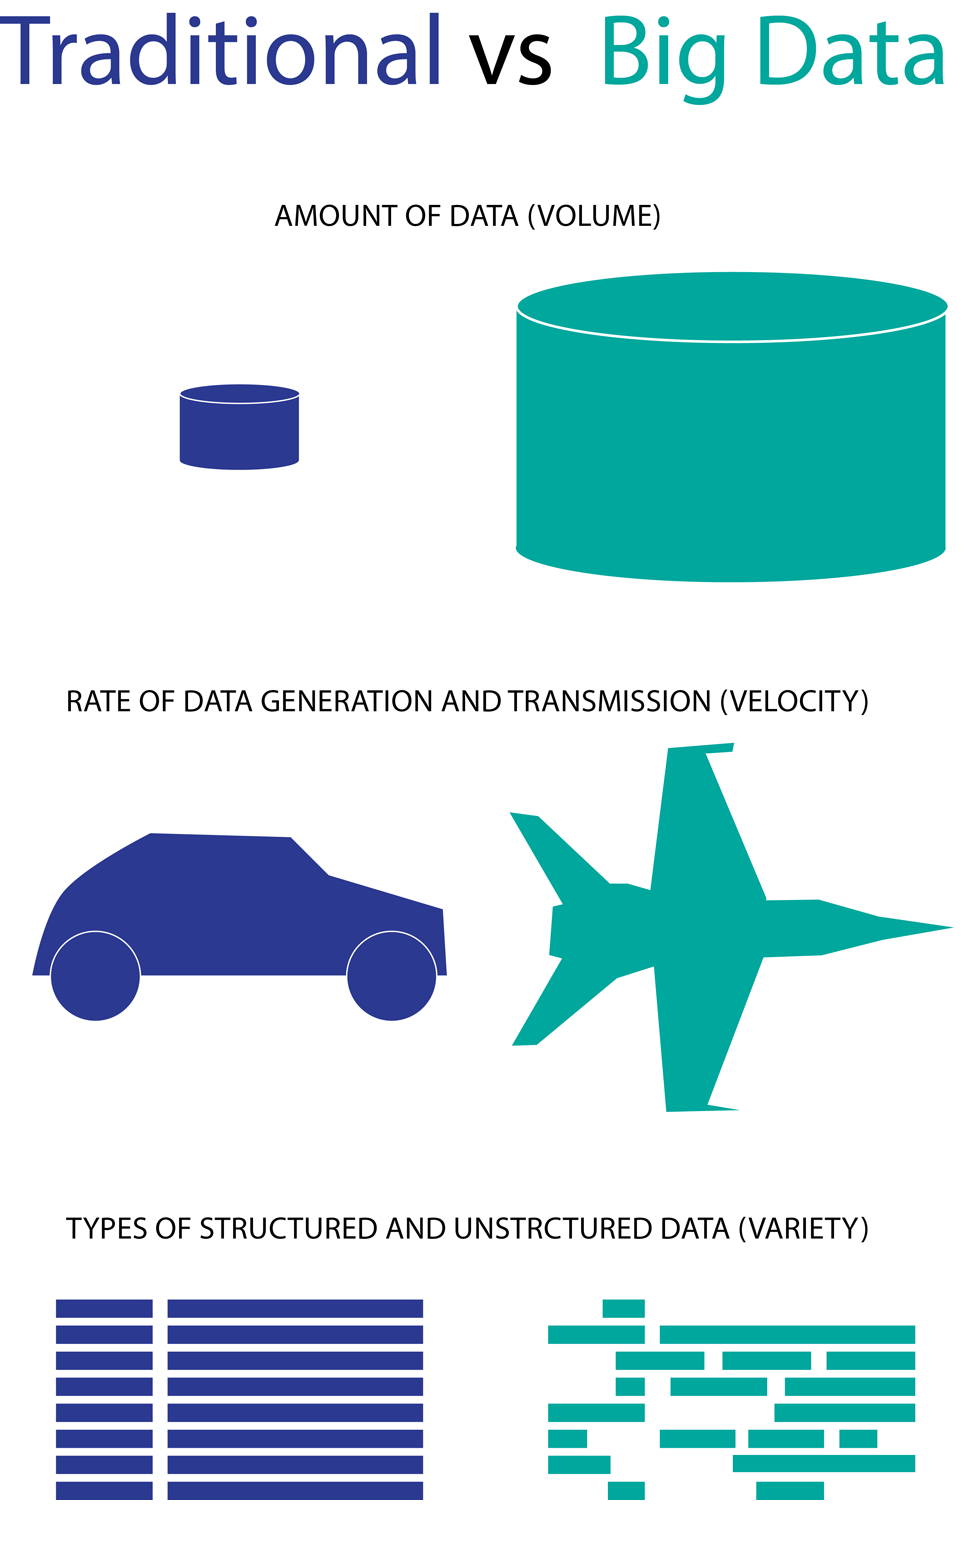
\includegraphics[width=\textwidth]{3keys.png}
    \end{column}

  \end{columns}
\end{frame}



\begin{frame}{Structured data Vs Semi-Structured Data}{Data formats}

  \begin{columns}

    \begin{column}{0.5\textwidth}
      \textbf{Structured Data}

      \vspace{0.5cm}

      \centering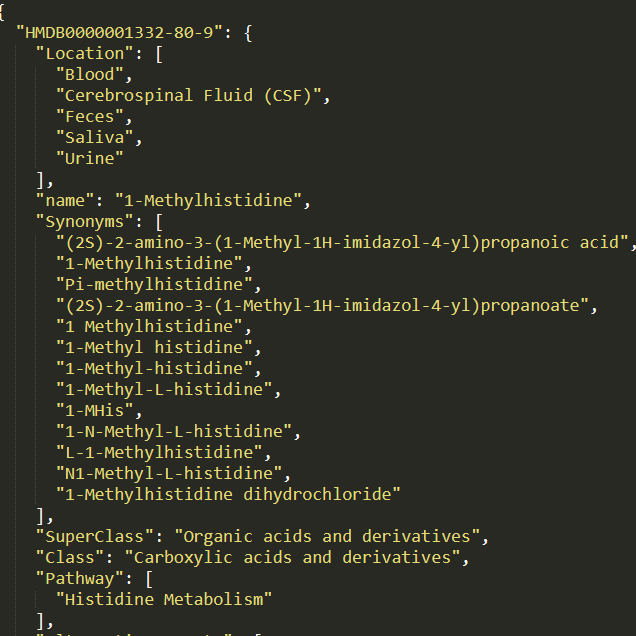
\includegraphics[width=\textwidth]{structured.png}
    \end{column}

    \begin{column}{0.5\textwidth}
      \textbf{UnStructured Data}

      \vspace{0.85cm}

      \centering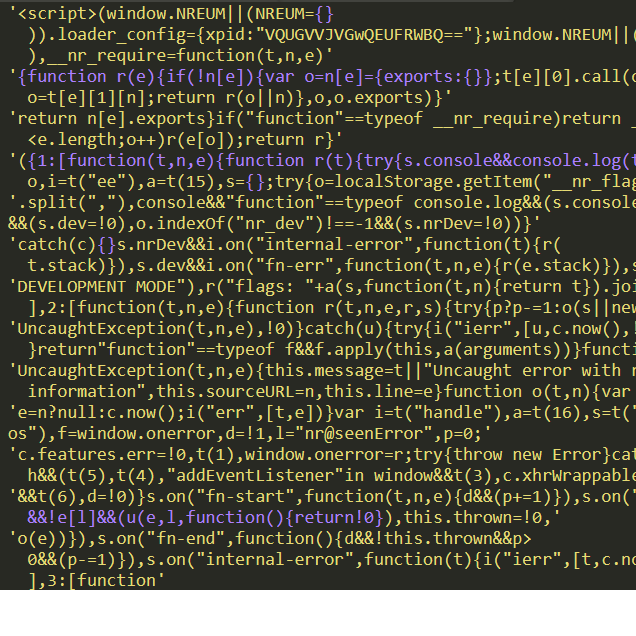
\includegraphics[width=\textwidth]{unstructured.png}
    \end{column}

  \end{columns}

\end{frame}


\begin{frame}{Web Scraping Algorithm}{Mining the Web}

  \textbf{Web scraping}, \textbf{web harvesting}, or web data extraction is data scraping used for extracting data from websites.

  \begin{columns}
    \begin{column}{0.3\textwidth}
      \centering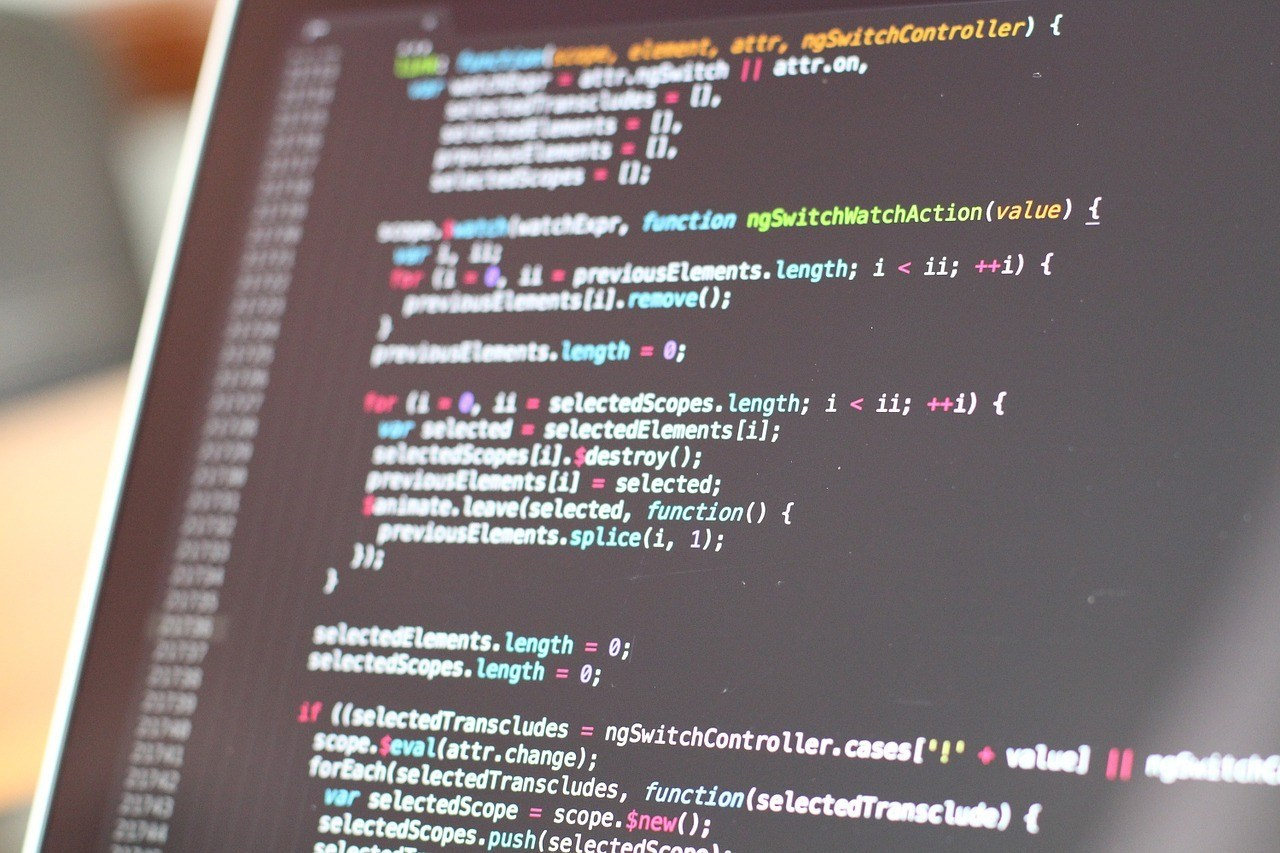
\includegraphics[width=\textwidth]{code.jpg}
    \end{column}
    \begin{column}{0.7\textwidth}
      \centering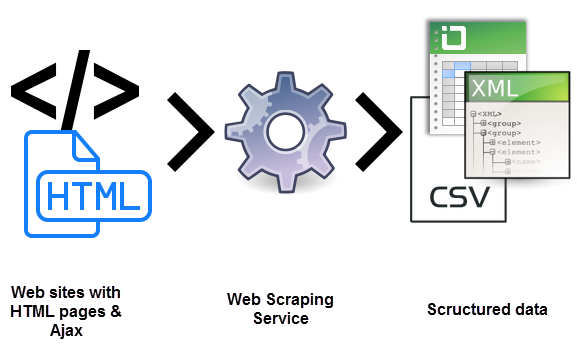
\includegraphics[width=\textwidth]{web-scraping-service.png}
    \end{column}
  \end{columns}

\end{frame}


\begin{frame}{FiloBLU Project}{A INFN project}

  \centering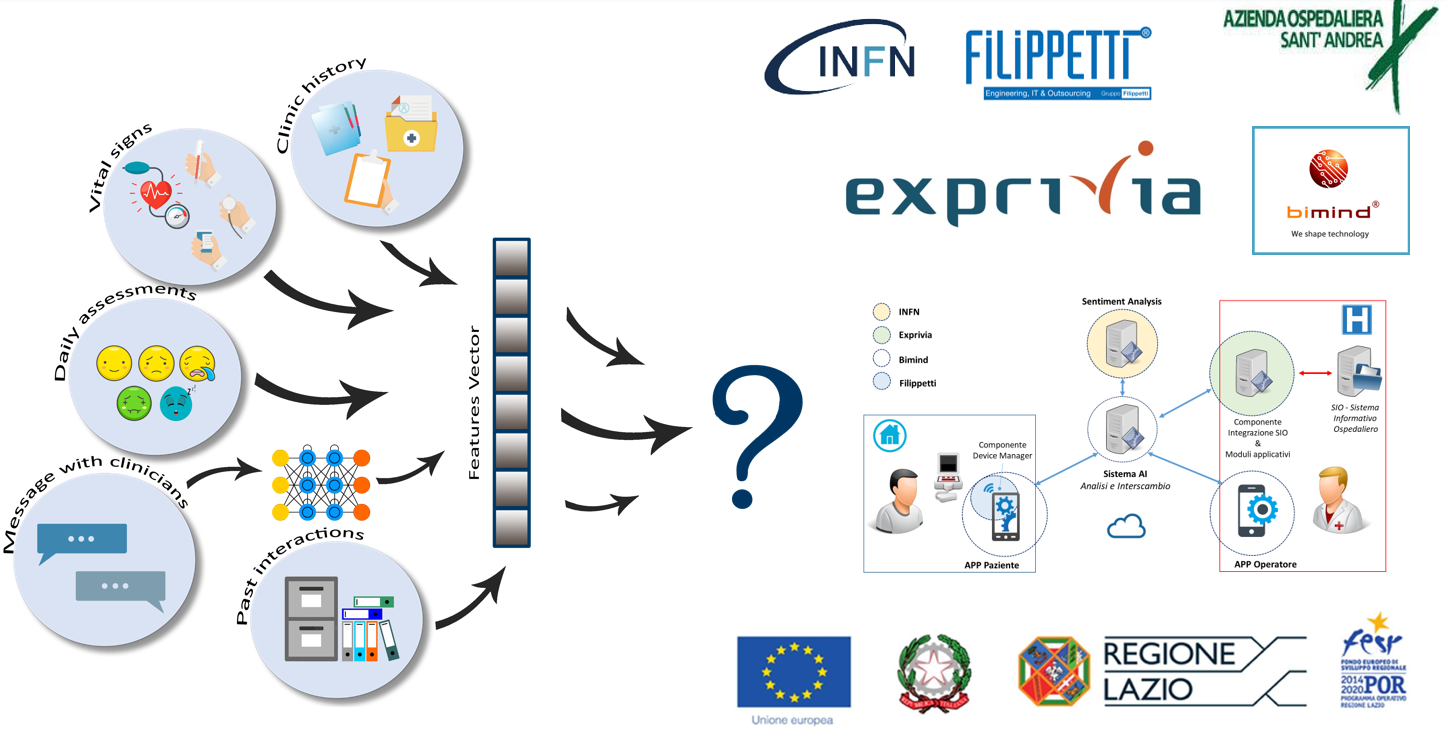
\includegraphics[width=\textwidth]{filoblu.png}

\end{frame}


\begin{frame}{Disease Ontology}{Sympotms Network}

  \setbeamertemplate{itemize items}[ball]
  \setbeamertemplate{itemize/enumerate body begin}{\scriptsize}
  \setbeamertemplate{itemize/enumerate subbody begin}{\scriptsize}

  \begin{columns}

    \begin{column}{0.4\textwidth}
      \centering
\includegraphics[width=\textwidth]{symptoms.png}

      \textbf{Symptoms Network:}
      \begin{itemize}
        \setlength\itemsep{1em}

        \item \textbf{nodes:} 2285;
        \item \textbf{links:} 29557;
      \end{itemize}

    \end{column}

    \begin{column}{0.6\textwidth}
      \centering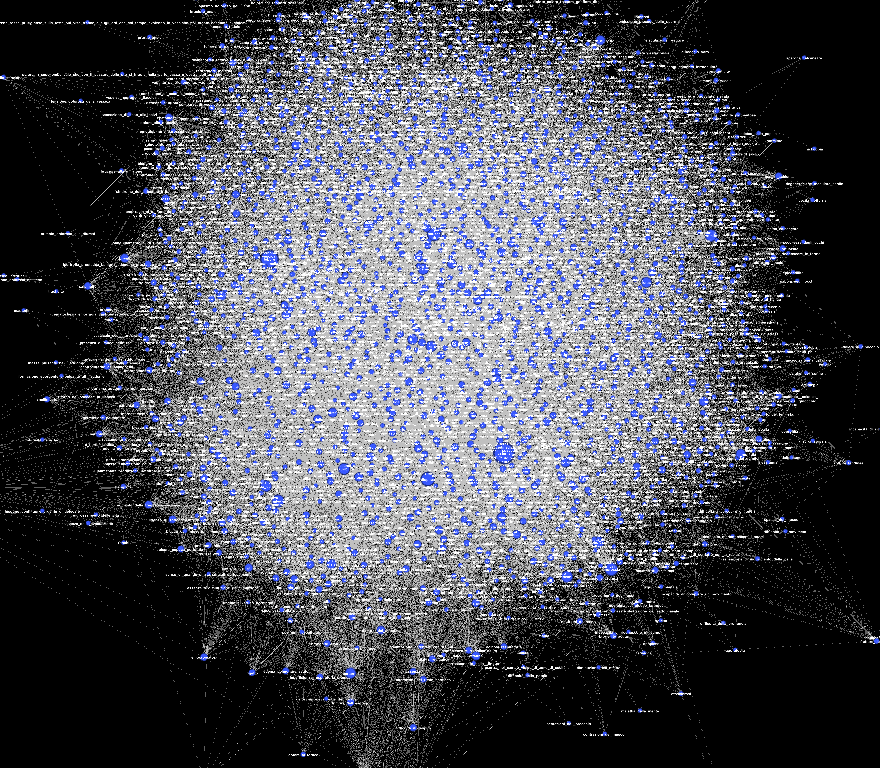
\includegraphics[width=\textwidth]{symnet.png}
    \end{column}

  \end{columns}

\end{frame}


\begin{frame}{Why CHIMeRA?}

  \setbeamertemplate{itemize items}[ball]
  \setbeamertemplate{itemize/enumerate body begin}{\scriptsize}
  \setbeamertemplate{itemize/enumerate subbody begin}{\scriptsize}
  \setbeamercolor{block title alerted}{fg=black, bg=darkred!40!white}
  \setbeamercolor{block body alerted}{fg=black, bg=white}

  \begin{alertblock}{Issues}
    \begin{itemize}

      \setlength\itemsep{2em}

      \item \textbf{Abysmal overlap between existing databases using medical ontology}.

      \item \textbf{Difficulties in propagating existing information between bipartite networks containing diseases}.

      \item \textbf{To find a way to let different type of information \quotes{talk} to each other through diseases}.

    \end{itemize}
  \end{alertblock}

\end{frame}


\begin{frame}{CHIMeRA Structure}{Data sources interaction}

  \centering The 6 most popular bio-medical databases:

  \centering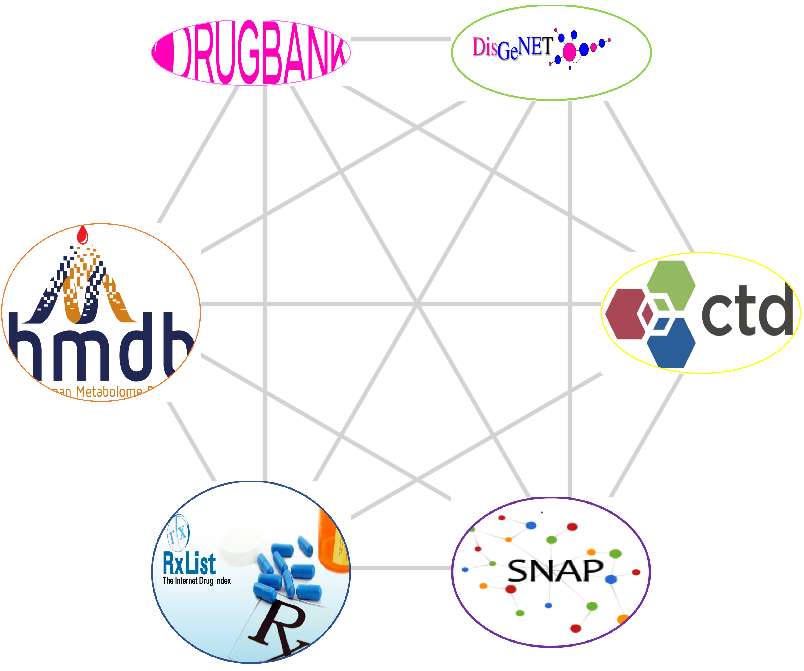
\includegraphics[width=0.7\textwidth]{CHIMeRA_loghi.png}

\end{frame}


\begin{frame}{Mining the Web}{Database contents}

  \begin{figure}
    \begin{overprint}
      \onslide<1>\centering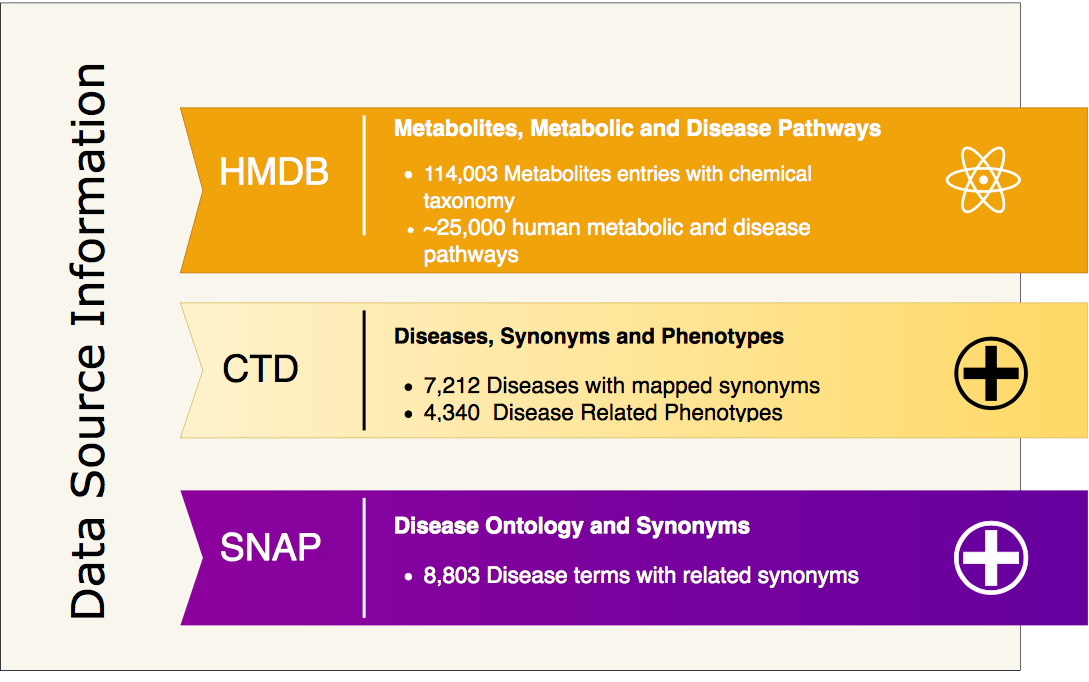
\includegraphics[width=\textwidth]{Chimera_db_sources1.png}
      \onslide<2>\centering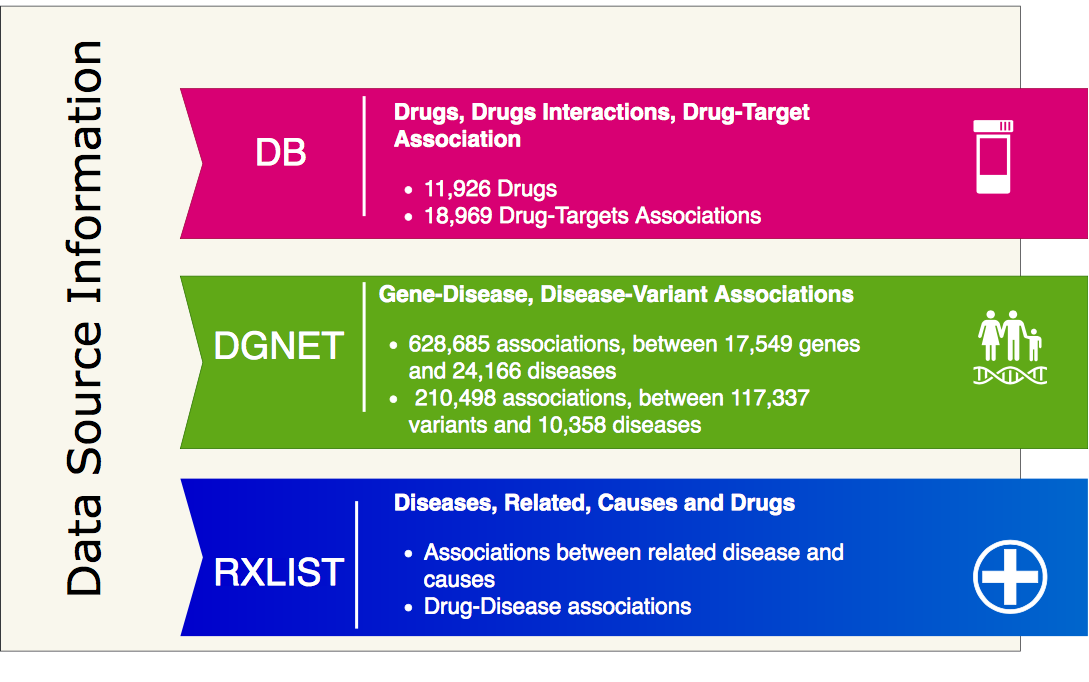
\includegraphics[width=\textwidth]{Chimera_db_sources2.png}
    \end{overprint}
  \end{figure}

\end{frame}



\begin{frame}{String Processing}{Pre-processing Pipeline}

  \centering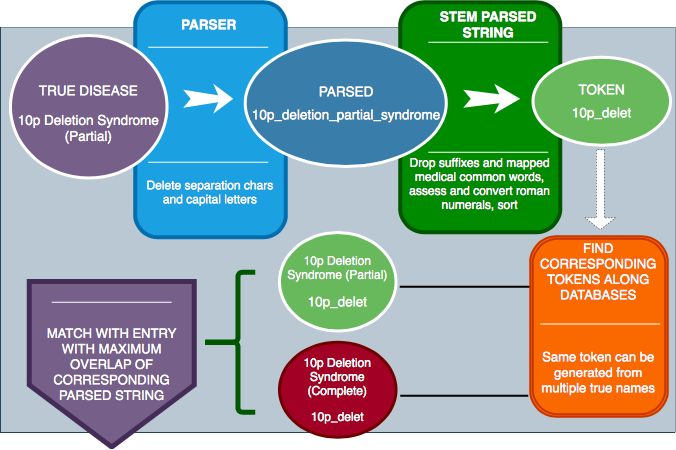
\includegraphics[width=0.9\textwidth]{chimera_pipeline.png}

\end{frame}


\begin{frame}{CHIMeRA}{Network visualization}
  \centering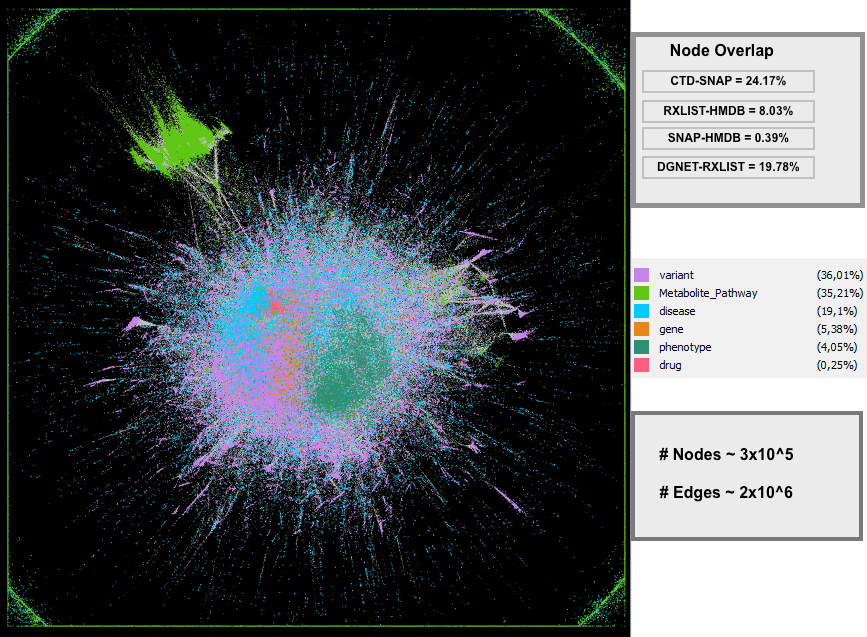
\includegraphics[width=0.9\textwidth]{chimera_plot-side_over_node.png}
\end{frame}


\begin{frame}{Preliminary Analysis}{Degree distributions}

  \centering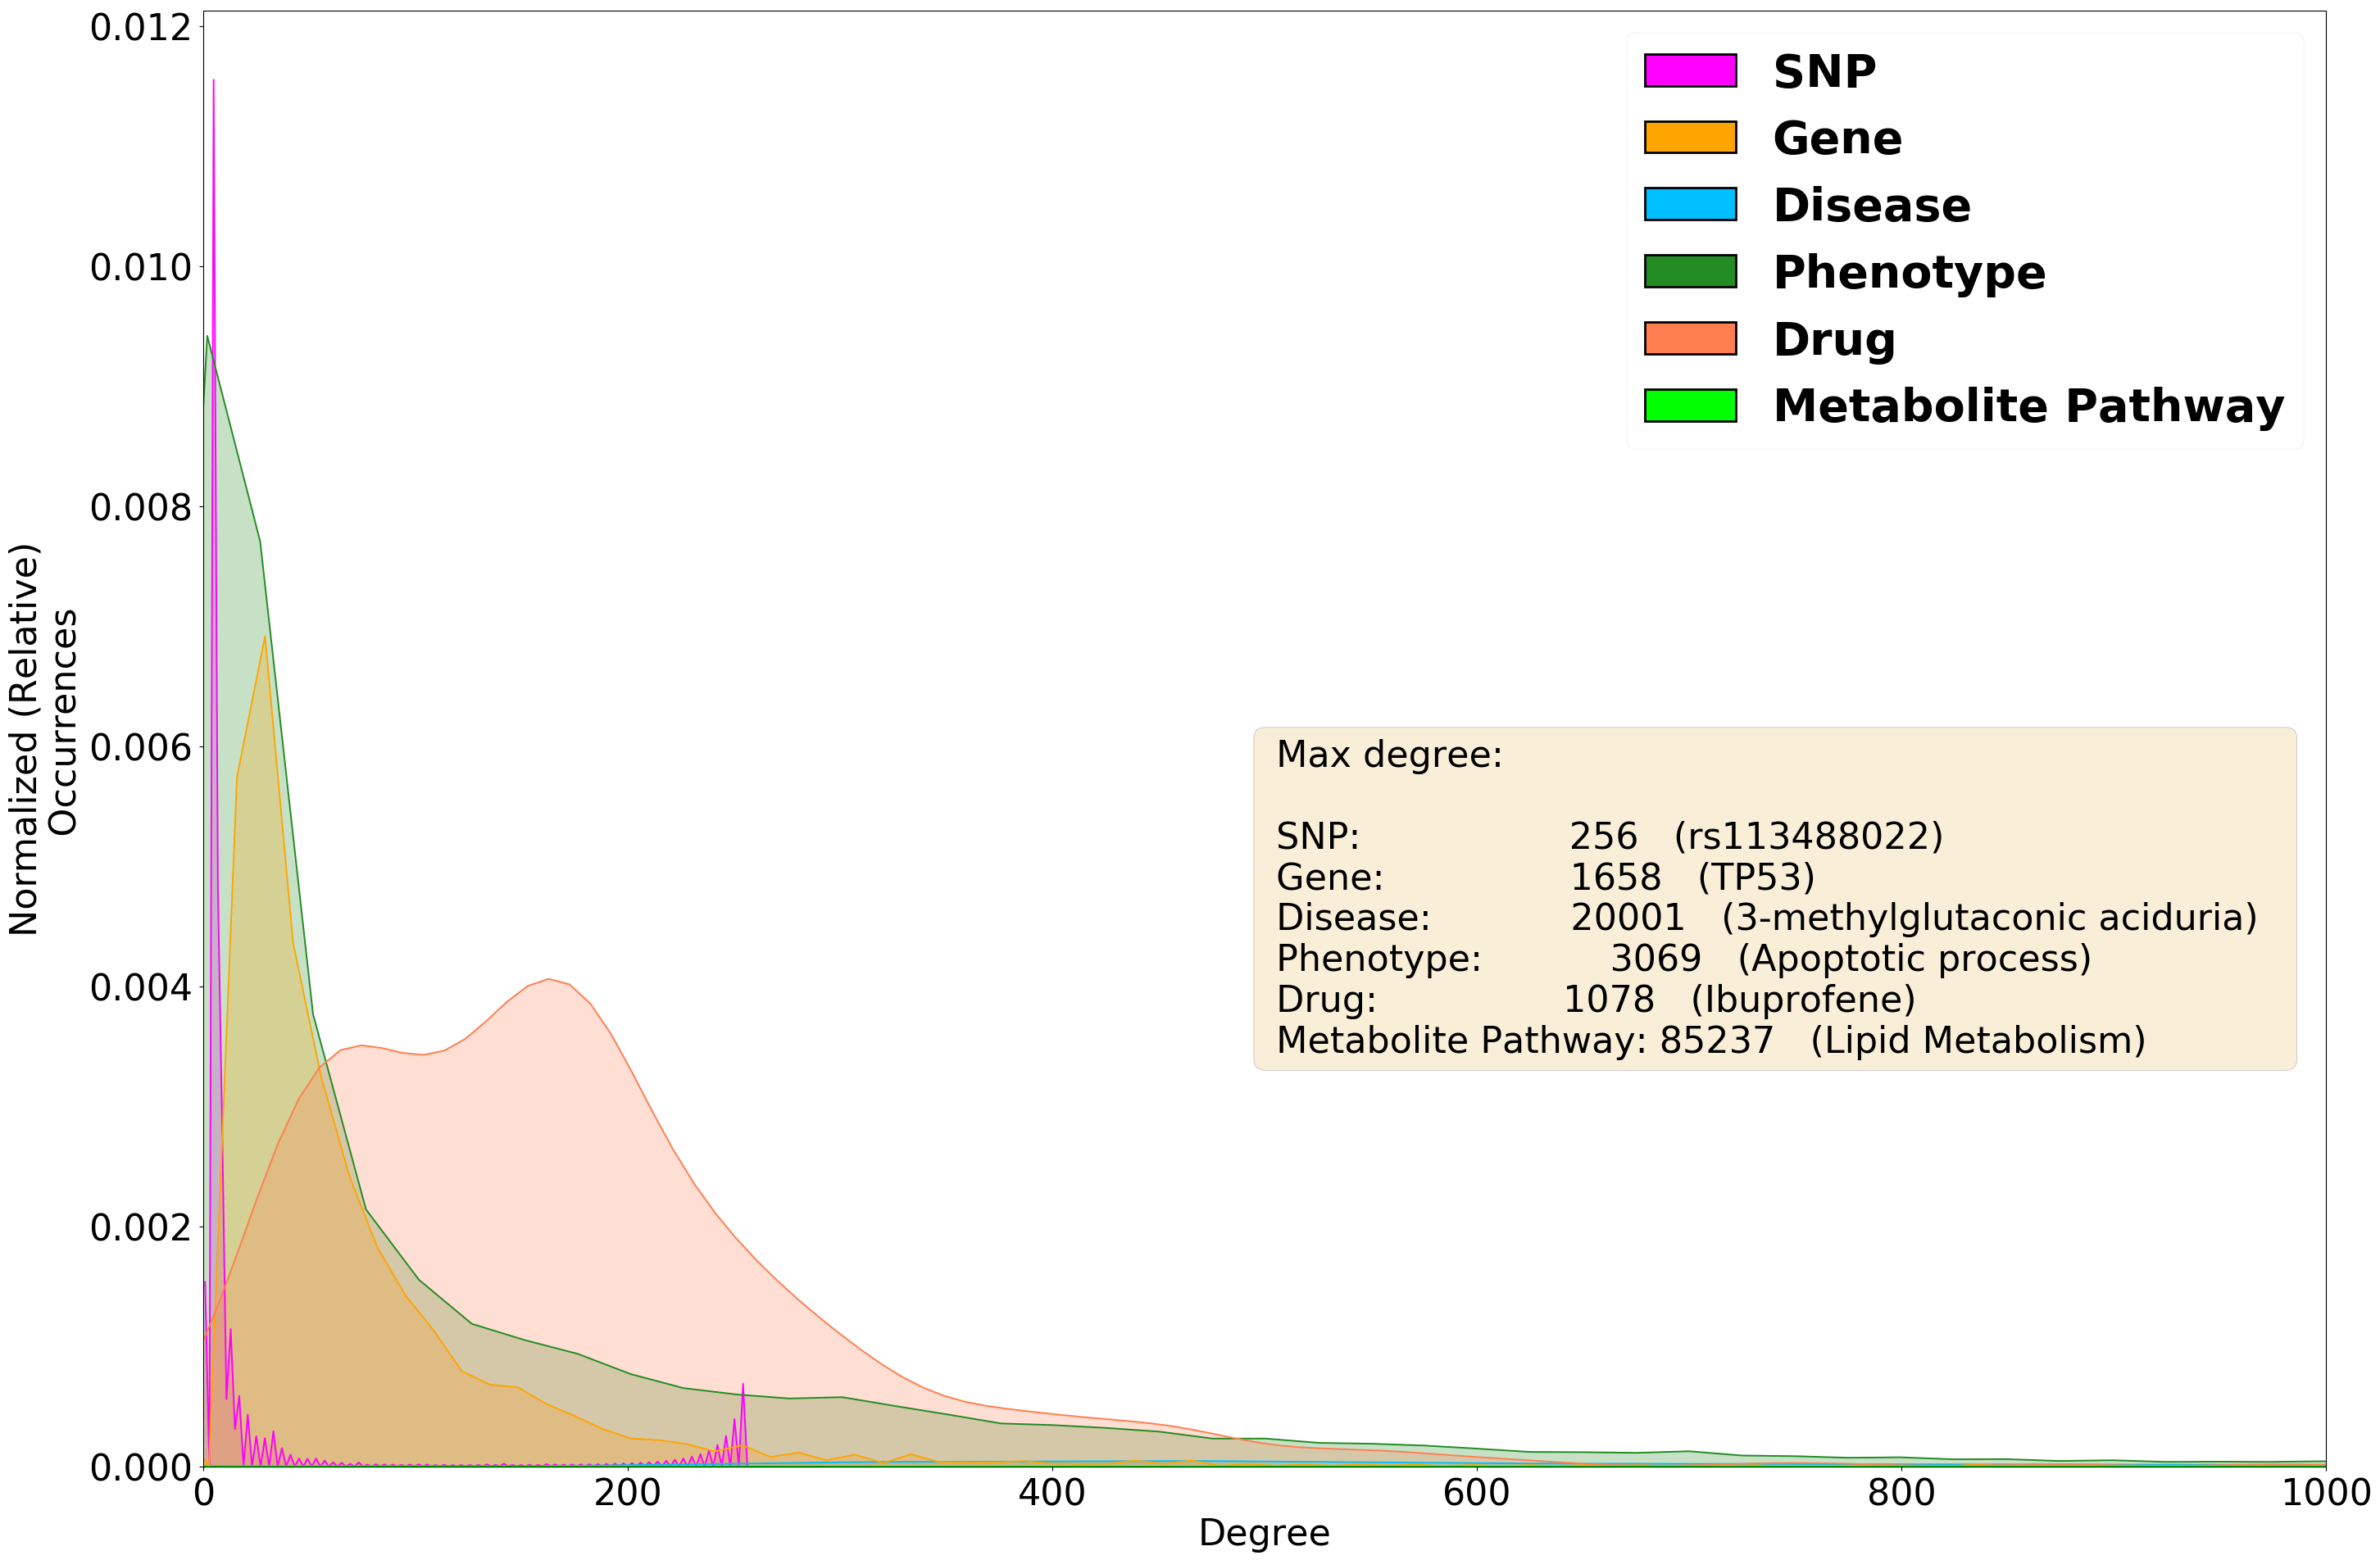
\includegraphics[width=0.95\textwidth]{degree.png}

\end{frame}


\begin{frame}{CHIMeRA as Service}

  \setbeamertemplate{itemize items}[ball]
  \setbeamertemplate{itemize/enumerate body begin}{\scriptsize}
  \setbeamertemplate{itemize/enumerate subbody begin}{\scriptsize}

  \centering CHIMeRA database: $\sim 3.6\times10^5$ nodes, $\sim 3.8\times10^7$ links

  \begin{block}

    \begin{itemize}
      \setlength\itemsep{2em}

      \item Convert Network structure to quearable DataBase (\textbf{ArangoDB});

      \item Search node according to its type (disease, gene, snp, ...):
        \begin{itemize}
          \setlength\itemsep{1em}
          \item Star graph: equivalent to single database search;
          \item Breath first search: percolation from a given root node;
          \item Multiple roots search: features intersection between nodes \textbf{(work in progress)};
          \item Shortest paths: minimum number of connections between two entries \textbf{(work in progress)}.
        \end{itemize}

      \item Graphical visualization of resulting networks: visual interaction between entries;

    \end{itemize}

  \end{block}

\end{frame}


\begin{frame}{Example 1}{Leukemia disease}

  \setbeamertemplate{itemize items}[ball]
  \setbeamertemplate{itemize/enumerate body begin}{\scriptsize}
  \setbeamertemplate{itemize/enumerate subbody begin}{\scriptsize}

  \begin{columns}
    \begin{column}{0.4\textwidth}
      Looking for \quotes{Leukemia} disease into CHIMeRA db:

      \begin{itemize}
        \setlength\itemsep{0.5em}
        \item 291 types of Leukemia;
        \item 82 connected components!
        \item 5270/9460 pendant nodes;
      \end{itemize}

      Fraction of types:

      \begin{itemize}
        \item 838 diseases;
        \item 2463 genes;
        \item 5195 phenotypes;
        \item 765 SNPs;
        \item 154 metabolite pathways;
        \item 40 metabolites;
        \item 5 drugs;

      \end{itemize}
    \end{column}

    \begin{column}{0.6\textwidth}
      \centering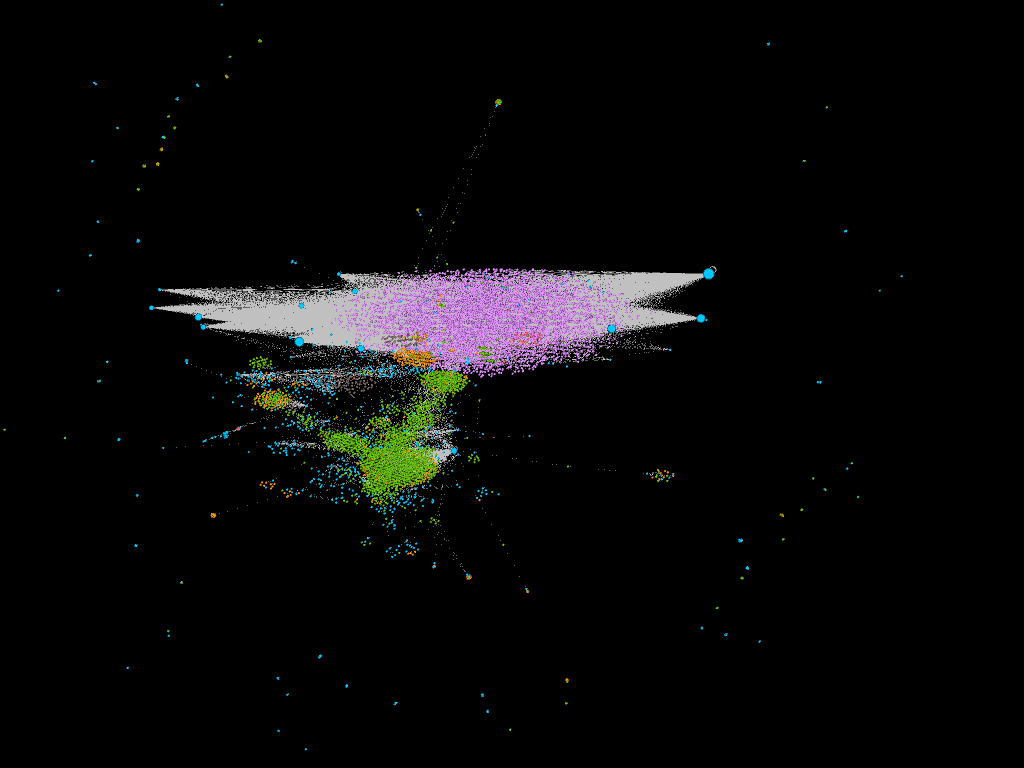
\includegraphics[width=\textwidth]{leukemia.png}
    \end{column}
  \end{columns}

\end{frame}


\begin{frame}{Example 2}{PRNP gene}

  \setbeamertemplate{itemize items}[ball]
  \setbeamertemplate{itemize/enumerate body begin}{\scriptsize}
  \setbeamertemplate{itemize/enumerate subbody begin}{\scriptsize}

  \begin{columns}
    \begin{column}{0.4\textwidth}
      Looking for \quotes{PRNP} gene into CHIMeRA db:

      \begin{itemize}
        \setlength\itemsep{0.5em}
        \item 1 types of PRNP;
        \item 1 connected component;
        \item 19103 nodes;
        \item 139496 links;
      \end{itemize}

      Fraction of types:

      \begin{itemize}

        \item 777 diseases;
        \item 9 drugs;
        \item 10452 genes;
        \item 1 metabolites;
        \item 576 pathways;
        \item 3775 phenotypes;
        \item 3513 SNPs;

      \end{itemize}
    \end{column}

    \begin{column}{0.5\textwidth}
      \centering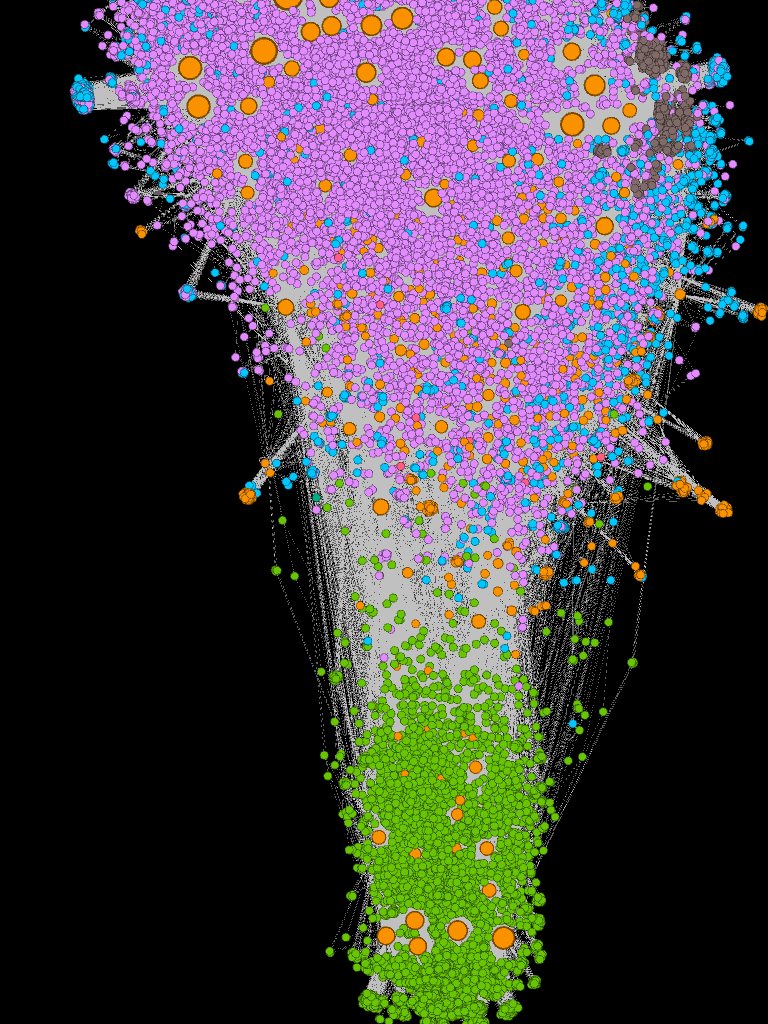
\includegraphics[width=0.9\textwidth]{prnp.png}
    \end{column}
  \end{columns}

\end{frame}


\begin{frame}{Work in Progress}{Next steps}

  \setbeamertemplate{itemize items}[ball]
  \setbeamertemplate{itemize/enumerate body begin}{\scriptsize}
  \setbeamertemplate{itemize/enumerate subbody begin}{\scriptsize}
  \setbeamercolor{block title}{fg=black, bg=NormalBlue}
  \setbeamercolor{block body}{fg=black, bg=white}

  \begin{block}{Future aims}

    \begin{itemize}
      \setlength\itemsep{2em}
      \item New build based on enhanced processing to increase information overlap.

      \item New features and information embedding from DrugBank and other data sources.

      \item Network of Networks analysis.

      \item Improve query efficiency and user interface.

      \item Release of the first public version as web service.
    \end{itemize}

  \end{block}

\end{frame}

\begin{frame}{Conclusions}{CHIMeRA project}

  \setbeamertemplate{itemize items}[ball]
  \setbeamertemplate{itemize/enumerate body begin}{\scriptsize}
  \setbeamertemplate{itemize/enumerate subbody begin}{\scriptsize}
  \setbeamercolor{block title}{fg=black, bg=NormalBlue}
  \setbeamercolor{block body}{fg=black, bg=white}

  \begin{itemize}
    \setlength\itemsep{2em}
    \item Interesting information seems to emerge from CHIMeRA, even at its alpha stage.

    \item Observational studies can be supported and observational biases mitigated by multi-level information patterns in the network.

    \item The goal is to propagate information using diseases as a \quotes{bridge}.

  \end{itemize}

\end{frame}


\end{document}
